% Created 2020-12-22 二 23:19
% Intended LaTeX compiler: xelatex
\documentclass[11pt]{report}
\usepackage{graphicx}
\usepackage{grffile}
\usepackage{longtable}
\usepackage{wrapfig}
\usepackage{rotating}
\usepackage[normalem]{ulem}
\usepackage{amsmath}
\usepackage{textcomp}
\usepackage{amssymb}
\usepackage{capt-of}
\usepackage{hyperref}
\author{曹嘉祺 PB18030874 化学与材料科学学院 有机化学系 \thanks{中国 安徽合肥 中国科学技术大学 Email: \href{mailto:mkq@mail.ustc.edu.cn}{mkq@mail.ustc.edu.cn}}}
\usepackage[scheme=plain]{ctex}
\usepackage{fontspec}
\usepackage[section]{placeins}
\setmainfont{更纱黑体 UI SC}
\hypersetup{colorlinks=true,linkcolor=blue}
\usepackage{longtable}
\date{\today}
\title{双液系的气液平衡相图}
\hypersetup{
 pdfauthor={曹嘉祺 PB18030874 化学与材料科学学院 有机化学系},
 pdftitle={双液系的气液平衡相图},
 pdfkeywords={},
 pdfsubject={},
 pdfcreator={Emacs 27.1 (Org mode 9.4)}, 
 pdflang={English}}
\begin{document}

\maketitle
\tableofcontents

\begin{abstract}
正丙醇-水是完全互溶体系,在本实验中用沸点仪测定出在一个大气压下,不同浓度的正丙醇-水双液体系的沸点, 并且用数字阿贝折射仪确定双液体系的恒沸混合物的组成,
得到正丙醇-水双液体系的气液平衡相图。


\noindent\rule{\textwidth}{0.5pt}
\begin{itemize}
\item 关键词: 气液平衡\quad 相图\quad 最低恒沸点
\end{itemize}
\end{abstract}
\begin{abstract}
 This experiment measured the phase diagram of a two-component system, the
n-polyalcohol-water system in a certain press. Then uses refractometer to draw the phase diagram,
and according to the phase diagram to work out the minimum constant boiling point. Master how
to use refractometer.


\noindent\rule{\textwidth}{0.5pt}

\begin{itemize}
\item key words: phase diagram of the binary liquid system, refractive index,  water-n-propyl alcohol system, the lowest boiling temperature
\end{itemize}
\end{abstract}
\part{前言}
\label{sec:orgb9eaa66}
\chapter{实验原理}
\label{sec:orgd413a35}
常温下的双液系有的只能部分互溶,有的则能完全互溶。本实验所用的水-正丙醇
双液系是完全互溶的。双液系的沸点与外压和其组成有关,且其气相和液相的组成一般不同。
通常用几何作图的方法将双液系的沸点对其气相和液相的组成作图,得到双液系的 T-x 相
图。完全互溶双液系在恒定压力下的气液平衡相图可分为三类, Fig 1.1 :

\begin{itemize}
\item 理想溶液,满足拉乌尔定律。
\item 实际溶液,偏离拉乌尔定律较远,具有最低恒沸点。
\item 实际溶液,偏离拉乌尔定律较远,具有最高恒沸点。
\end{itemize}
\begin{figure}[htbp]
\centering
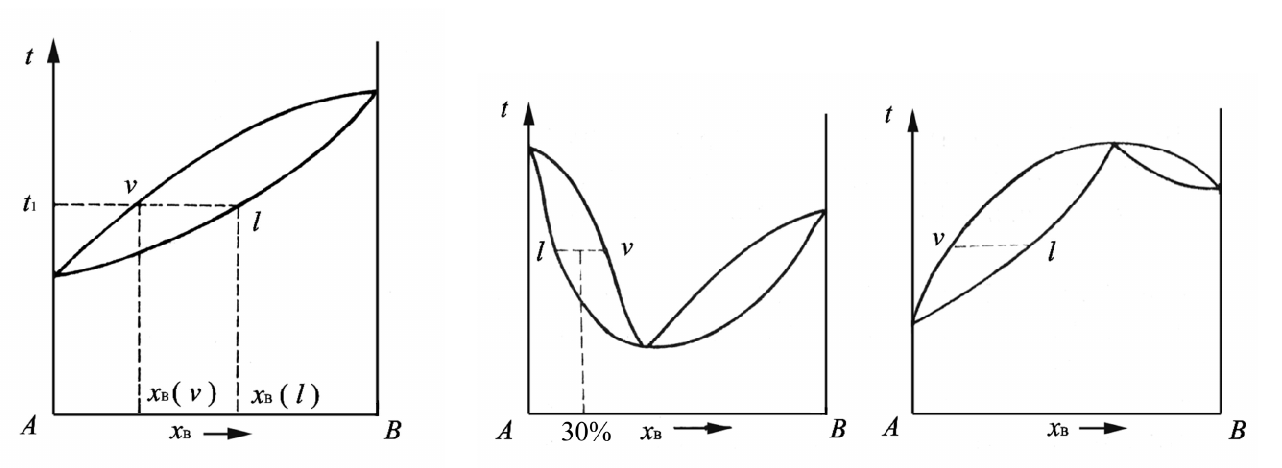
\includegraphics[width=.9\linewidth]{../img/1.png}
\caption{\label{fig:org7519021}三种溶液的相图}
\end{figure}
正丙醇-水等体系具有最低恒沸点,为第二类。

本实验两相中的成分分析均采用折射率法,通过测折光率的大小在工作曲线上找出未知
溶液的浓度与组成,从而画出体系的相图。

沸点的测定:用玻璃水银温度计测量溶液的沸点,需作两种校正:
\section{露茎校正}
\label{sec:orgdea0b56}
    这是由于温度计未能完全置于被测体系中而引起的。根据玻璃与水银膨胀系数的差异,校正值的计算式是:
\[
\Delta t_{露}=1.6\times 10^{-4}\cdot n \cdot (t_{观}-t_{环})
\]
式中的 n 是露出的那段水银柱的长以温度差作为单位,1.6\texttimes{} 10\textsuperscript{-4} 是水银对玻璃的相对膨胀系数。
但本次实验所用温度计是数显的电子温度计,所以以上操作实际上并没有做
\section{压力校正}
\label{sec:orgd1f7c84}
    标准大气压下(P=760mmHg,即 101325Pa)测得的沸点为正常沸点。应用特鲁顿规则及克劳修斯-克拉贝龙公式,可得溶液沸点随大气压变动而变动的近似值为:
\[
\Delta t_{压}=\frac{273.15+t_{观}}{10}\cdot \frac{101325-P}{101325}
\]
校正后,溶液的正常沸点为:
\[
t_{沸}=t_{观}+\Delta t_{压}+\Delta t_{露}
\]



\part{实验部分}
\label{sec:org7646880}
\chapter{实验仪器与试剂}
\label{sec:orge4581be}
\section{仪器}
\label{sec:org1290668}
实验所用的仪器如Tab 2.1 所示
\begin{table}[htbp]
\caption{\label{tab:org4d7b709}实验仪器}
\centering
\begin{tabular}{lll}
仪器 & 数目 & 备注\\
\hline
沸点仪 & 1套 & \\
阿贝折射仪 & 1台 & 上海申光仪器仪表有限公司\\
精密稳流电源调压变压器 & 1支 & 南大万和\\
加热套 & 1台 & \\
加热电阻丝 & 1支 & \\
电子温度计 & 1台 & \\
移液管 & 3支 & 20mL,50mL,10mL\\
干燥吸管 & 若干 & 包含长短两种\\
擦镜纸 & 一包 & \\
正丙醇 & 一瓶 & \\
蒸馏水 &  & \\
\end{tabular}
\end{table}

\chapter{实验步骤}
\label{sec:org86c2513}
\section{安装沸点仪}
\label{sec:org25df143}
将烘干的沸点仪安装好。
\section{测正丙醇的沸点}
\label{sec:orge97d65e}
     用 50mL 的移液管从支管 L 中加入正丙醇溶液 50mL,夹上电热丝夹,
打开冷却水,插上电源,调节变压器电压由零慢慢增加,观察加热丝上是否有小气泡逸出,
电压控制在 15V 以内,保温套电压控制在150V以内,溶液会慢慢沸腾。
体系中的蒸汽经冷凝管冷凝后,聚于小球 D 中。冷
凝液不断地冲刷 D 球,必要时可将 D 球中的冷凝液吸入烧瓶中,观察 B 温度计上的读数达到
稳定,此时体系处于平衡状态;再稳定 5-7 分钟,准确记下温
度计示数,测三次。切断电源。
\section{取样并测定折光率}
\label{sec:org36001f4}
     用干燥的滴定管自冷凝管中取出小球 D 内的全部气相冷凝液,用另
一支干燥吸管从 L 口中取液相液 1mL 左右,分别放入小试管中,并将试管置于一
盛有冷水的小烧瓶中让其冷却。观察阿贝折射仪上的温度是否正确。用无尘纸擦拭镜面,
把待测的气相液,液相液分别滴于镜面上迅速测量。每个样品测量 1 次 。
\section{加入水后进行测量}
\label{sec:orgeac73fc}
    用 10mL 移液管移取 H2O 0.5 mL,从支管 L 加入烧瓶中,以改变溶液的总组成,按步骤 2
-3 测量新体系中的液相、气相的折光率和平衡时的 t 。依次向烧瓶中加入 1,1.5,
2,2.5,4mL 的水,仍按步骤 2-3 逐一进行测量,分别得到不同组成时的气相、液相的
折光率及各自的沸点。
\section{查出组成}
\label{sec:orgfb12a83}
由以上测得的各个气相、液相样品的折光率,从工作曲线上查找出其对应的组成。



\chapter{实验数据及数据处理(见附件)}
\label{sec:org5dfb97b}
\chapter{结果分析与讨论}
\label{sec:org99030a7}
\section{实验结果}
\label{sec:org4429876}
\begin{enumerate}
\item 标准曲线
\label{sec:orgad5568a}
经过对标准曲线的绘制 Fig 5.1 , 我们利用对数函数拟合数据得到了
摩尔分数和折光率之间的对应关系,虽然也尝试了其他的拟合方式,但只有对数函数的拟合效果最佳
\[
y=0.01464\ln(1.5835x+0.03743)+1.3794
\]
其中y表示折光率,x表示正丙醇的摩尔分数
\begin{figure}[htbp]
\centering
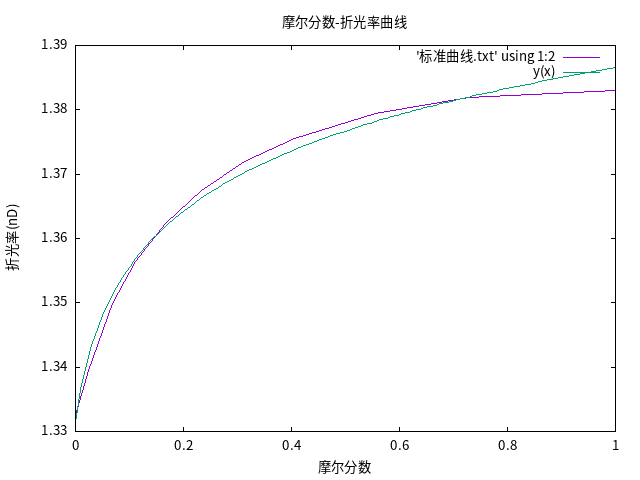
\includegraphics[width=.9\linewidth]{../data/标准曲线-对数曲线拟合.png}
\caption{对数曲线拟合结果}
\end{figure}
\item 气液相图绘制
\label{sec:orgc9b35cf}
利用特鲁顿规则及克劳修斯-克拉贝龙公式和前一节得到的关系式,
将所得的沸点数据根据大气压校正为标准值,计算出气液组分的摩尔分数,
根据沸点和气液组分摩尔分数进行绘图 Fig 5.2

 考虑到可能存在的坏点导致曲线并不平滑,采用bezier方法进行了平滑化,
得到了Fig 5.2 所示的结果,可以明显地看出其中的共沸点,数据处理效果良好

\begin{figure}[htbp]
\centering
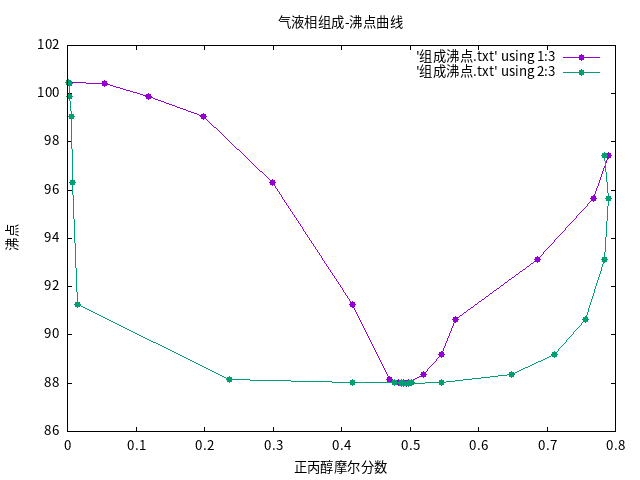
\includegraphics[width=.9\linewidth]{../data/气液相组成-沸点曲线.png}
\caption{水-正丙醇体系气液相图}
\end{figure}


\begin{figure}[htbp]
\centering
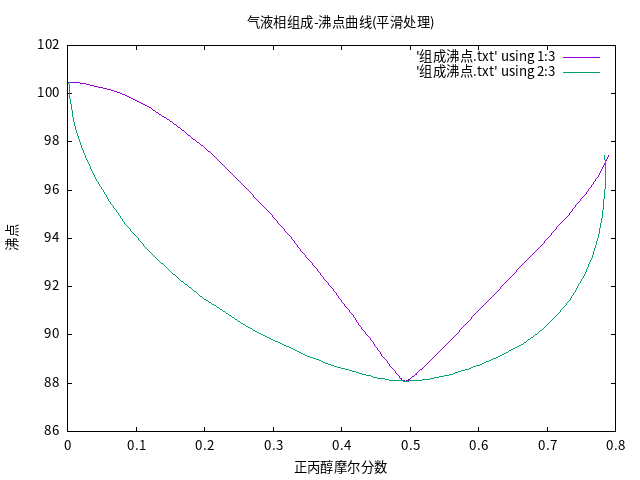
\includegraphics[width=.9\linewidth]{../data/气液相组成-沸点曲线(平滑处理).png}
\caption{水-正丙醇体系气液相图(平滑处理)}
\end{figure}
\item 结论
\label{sec:org90cb36e}
     不难看出水—正丙醇体系是属于正偏差很大的体系,可在 T\textasciitilde{}x 图上产生最低点,
该点即为最低恒沸点,在该点,体系的气液两相有共同的组成,该混合物不能通过蒸
馏加以分离。随着组成的不同,双液系的沸点是不一样的;正丙醇—水体系的液相与
气相的 T-x 相图是不一样的,证明了“一般情况下,双液系的液相与气相组成是不一
样的;虽然随着组成的改变,双液系的沸点也随着改变,但是总有一个最低值存在,
如上所说,即最低恒沸点。也说明了正丙醇—水体系属于第三类完全互溶体系。
由图不难读出可见最低恒沸点为87.98°C,
关于恒沸混合物含正丙醇的质量百分比为
71.82\%。书中给出最低恒沸点为:87°C
 正丙醇的质量百分比为69\%-71\%。实验值与理论值略有偏差。
\end{enumerate}

\section{实验讨论}
\label{sec:org5f8687f}
\begin{enumerate}
\item 误差分析
\label{sec:org51d3dd1}
\begin{enumerate}
\item 本实验实际为两个人合作完成。由于各人的操作习惯、读数习惯和实验所用仪器的不同,因此不可避免产生了误差。在最后所得的相图上可以看出,两部分的图像拟和得并不是很好。
\item 读温度时,体系未达到气液平衡,实验要求要平衡 6-7 分钟,但实际操作中往往没有平衡那么久,而且温度计读数在沸腾时总是有0.01°C左右的波动,故读数上也会有一定的误差。
\item 实验中有过热和分馏作用,且气相组分往往不能完全取出,会影响气相的浓度,造成误差。
\item 实验中所测量的数据偏少,做出的图线就相对粗糙。
\item 实验中参照的折光率——正丙醇——水双液系百分比工作曲线图,是手工绘制的,本身就存在误差,不可能很精确的读数。
\item 对于工作曲线拟合的函数选择也有一些问题,对数函数在曲线后半部分的拟合结果较差,如果有更加精确的拟合函数,实验的精度应该会有所提升
\item 平衡时,气液两相温度应该一样。但实际中,由于体系中气相和液相跟环境的辐射和热对流的情况不同,所以实际温度,二者是不同的。这对测量将造成影响,因为稳定时气相的温度比液相低,以此做出的图比真实图偏瘦,即气相部分下移。若出现过热,则使所测量的温度高于实际沸点,则相图上移。若有分馏作用,由于正丙醇为一挥发组分,则气相组分变高,液相组分变低,所以出现左半相图变胖,右半相图变瘦。与实际情况符合。
\item 由于各组分的引力不同,如水-正丙醇间的引力小于水-水或正丙醇-正丙醇间的引力,则把正丙醇分子掺入后就会减少水分子或正丙醇分子所受的引力,水和正丙醇都变得很容易逸出,所以水或正丙醇分子的蒸汽压都产生正偏差,如实验所得结果。
\end{enumerate}
\item 实验反思
\label{sec:org5ce5199}
\begin{enumerate}
\item 由于在正丙醇的量相对来说很少的时候,测量值与以后的各值在进行拟合时不容易拟合,所以应当在开始加入正丙醇(或水)时适当多测量几组数据,使得在做图时较为容易与准确
\item 在反应时拔出塞子的时候,常因为冷却不充分导致有正丙醇蒸汽冒出,导致液相的组分发生变化,应当充分冷却后再取下塞子
\end{enumerate}
\end{enumerate}


\part{参考文献}
\label{sec:org23b2405}
\begin{enumerate}
\item 崔献英,柯燕雄,单绍纯.物理化学实验[M].合肥:中国科学技术大学出版社,2000.4
\item 傅献彩,沈文霞,姚天扬.物理化学.第四版.北京:高等教育出版社,1990.10
\item 苏碧泉,盛 丽,刘改兰. 气液平衡相图绘制实验的改进.兰州:化学教育,2006.2
\item 刘一品,唐晖. 双液系的气液平衡相图实验装置的改进.武汉:大学化学,2003.12
\item 百度百科数据库.
\end{enumerate}

\part{附录: 数据处理过程}
\label{sec:org80f072a}
\chapter{原始数据}
\label{sec:orge83c704}
\section{压强记录}
\label{sec:orgbdc6681}
在实验的前中后分别读取室内的大气压 Tab 6.1
\begin{table}[htbp]
\caption{\label{tab:org75fc2af}压强记录}
\centering
\begin{tabular}{rr}
序号 & 压强(kPa)\\
\hline
1 & 103.30\\
2 & 103.34\\
3 & 103.33\\
\hline
平均 & 103.323\\
\end{tabular}
\end{table}

\section{标准曲线的标定}
\label{sec:org5ac83e5}
测试一组不同浓度的正丙醇溶液的折光率 Tab 6.2
\begin{table}[htbp]
\caption{\label{tab:orgec5feee}标准曲线数据}
\centering
\begin{tabular}{rrrrrrr}
序号 & 空瓶(g) & 加水(g) & 加醇(g) & 水重(g) & 醇重(g) & 折光率(nD)\\
\hline
1 & 24.1634 & 33.1235 & 33.8728 & 8.9601 & 0.7493 & 1.3395\\
2 & 24.0538 & 31.9971 & 33.9486 & 7.9433 & 1.9515 & 1.3499\\
3 & 24.8590 & 31.8049 & 34.6950 & 6.9459 & 2.8901 & 1.3564\\
4 & 24.4442 & 30.4160 & 34.3886 & 5.9718 & 3.9726 & 1.3623\\
5 & 23.2520 & 28.1099 & 33.0280 & 4.8579 & 4.9181 & 1.3674\\
6 & 24.4106 & 28.3518 & 34.3383 & 3.9412 & 5.9865 & 1.3719\\
7 & 23.1017 & 26.1164 & 33.0016 & 3.0147 & 6.8852 & 1.3756\\
8 & 27.4522 & 29.3480 & 37.2448 & 1.8958 & 7.8968 & 1.3795\\
9 & 25.5501 & 26.5443 & 35.4334 & 0.9942 & 8.8891 & 1.3819\\
\end{tabular}
\end{table}
\section{醇加水的数据}
\label{sec:org082f90a}
向正丙醇中加水的气液相折光率数据 Tab 6.3
\begin{table}[htbp]
\caption{\label{tab:orgc53916a}醇加水的数据}
\centering
\begin{tabular}{rrrrrrr}
水(ml) & t\textsubscript{1}(\textsuperscript{o}C) & t\textsubscript{2}(\textsuperscript{o}C) & t\textsubscript{3}(\textsuperscript{o}C) & t\textsubscript{均}(\textsuperscript{o}C) & 气相(nD) & 液相(nD)\\
\hline
0.0 & 97.425 & 97.433 & 97.440 & 97.4327 & 1.3831 & 1.3830\\
0.5 & 95.667 & 95.671 & 95.680 & 95.6727 & 1.3827 & 1.3831\\
1.0 & 93.114 & 93.119 & 93.118 & 93.1170 & 1.3811 & 1.3830\\
1.5 & 90.666 & 90.650 & 90.659 & 90.6583 & 1.3784 & 1.3825\\
2.0 & 89.174 & 89.179 & 89.174 & 89.1757 & 1.3779 & 1.3816\\
2.5 & 88.349 & 88.355 & 88.356 & 88.3533 & 1.3772 & 1.3803\\
4.0 & 88.025 & 88.027 & 88.028 & 88.0267 & 1.3766 & 1.3779\\
2.0 & 88.004 & 88.007 & 88.008 & 88.0063 & 1.3765 & 1.3766\\
0.2 & 87.994 & 87.998 & 87.997 & 87.9963 & 1.3764 & 1.3764\\
0.2 & 87.977 & 87.984 & 87.987 & 87.9827 & 1.3764 & 1.3763\\
\end{tabular}
\end{table}
\section{水加醇的数据}
\label{sec:org76a0398}
向水中加正丙醇的气液相折光率数据 Tab 6.4
\begin{table}[htbp]
\caption{\label{tab:org61243eb}水加醇的数据}
\centering
\begin{tabular}{rrrrrrr}
醇(ml) & t\textsubscript{1}(\textsuperscript{o}C) & t\textsubscript{2}(\textsuperscript{o}C) & t\textsubscript{3}(\textsuperscript{o}C) & t\textsubscript{均}(\textsuperscript{o}C) & 气相(nD) & 液相(nD)\\
\hline
0.0 & 100.462 & 100.464 & 100.471 & 100.4657 & 1.3325 & 1.3325\\
0.5 & 100.421 & 100.425 & 100.425 & 100.4237 & 1.3488 & 1.3326\\
1.0 & 100.000 & 99.860 & 99.831 & 99.8970 & 1.3575 & 1.3327\\
1.5 & 99.024 & 99.099 & 99.051 & 99.0580 & 1.3641 & 1.3344\\
2.0 & 96.331 & 96.307 & 96.350 & 96.3293 & 1.3696 & 1.3354\\
4.0 & 91.237 & 91.265 & 91.281 & 91.2610 & 1.3741 & 1.3381\\
20.0 & 88.142 & 88.156 & 88.169 & 88.1557 & 1.3758 & 1.3664\\
15.0 & 88.017 & 88.023 & 88.027 & 88.0223 & 1.3762 & 1.3741\\
10.0 & 88.039 & 88.046 & 88.048 & 88.0443 & 1.3764 & 1.3767\\
1.0 & 88.034 & 88.036 & 88.042 & 88.0373 & 1.3764 & 1.3760\\
1.0 & 88.036 & 88.037 & 88.040 & 88.0377 & 1.3764 & 1.3763\\
\end{tabular}
\end{table}

\chapter{数据处理}
\label{sec:org79b80c8}
\section{标准曲线的绘制}
\label{sec:org1c55f15}
将Tab 6.2中的质量浓度换算成分子摩尔分数再加上纯物质的折光率数据得到Tab 7.1
\begin{table}[htbp]
\caption{\label{tab:org0c4b7be}标准曲线计算}
\centering
\begin{tabular}{rrrrr}
序号 & 水重(g) & 醇重(g) & 醇摩尔分数 & 折光率(nD)\\
\hline
0 &  &  & 0.0000 & 1.3325\\
1 & 8.9601 & 0.7493 & 0.0245 & 1.3395\\
2 & 7.9433 & 1.9515 & 0.0686 & 1.3499\\
3 & 6.9459 & 2.8901 & 0.1109 & 1.3564\\
4 & 5.9718 & 3.9726 & 0.1663 & 1.3623\\
5 & 4.8579 & 4.9181 & 0.2328 & 1.3674\\
6 & 3.9412 & 5.9865 & 0.3129 & 1.3719\\
7 & 3.0147 & 6.8852 & 0.4064 & 1.3756\\
8 & 1.8958 & 7.8968 & 0.5553 & 1.3795\\
9 & 0.9942 & 8.8891 & 0.7283 & 1.3819\\
10 &  &  & 1.0000 & 1.3830\\
\end{tabular}
\end{table}
\begin{enumerate}
\item 二次曲线拟合
\label{sec:orgf3faba9}
拟合结果见 Fig 7.1
\begin{figure}[htbp]
\centering
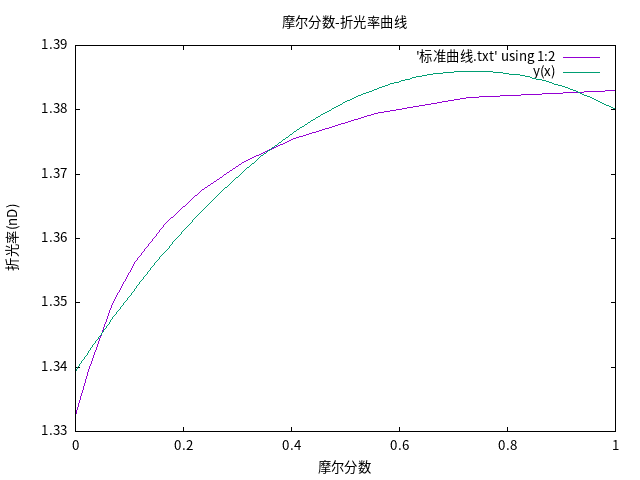
\includegraphics[width=.9\linewidth]{../data/标准曲线-二次曲线拟合.png}
\caption{\label{fig:orgb569b4b}二次曲线拟合结果}
\end{figure}
误差如下:
\begin{verbatim}
After 4 iterations the fit converged.
final sum of squares of residuals : 0.000147385
rel. change during last iteration : -3.6246e-08

degrees of freedom    (FIT_NDF)                        : 8
rms of residuals      (FIT_STDFIT) = sqrt(WSSR/ndf)    : 0.00429222
variance of residuals (reduced chisquare) = WSSR/ndf   : 1.84232e-05

Final set of parameters            Asymptotic Standard Error
=======================            ==========================
a               = -0.0861489       +/- 0.01461      (16.96%)
b               = 0.126901         +/- 0.0143       (11.27%)
c               = 1.33927          +/- 0.002455     (0.1833%)

correlation matrix of the fit parameters:
#                a      b      c      
a               1.000 
b              -0.955  1.000 
c               0.632 -0.773  1.000 

\end{verbatim}
\[
y=-0.08615x^{2}+0.1269x+1.3393
\]
拟合效果较好但仍有待提升
\item 对数曲线拟合
\label{sec:orge21dff5}
拟合结果见 Fig 7.2
\begin{figure}[htbp]
\centering
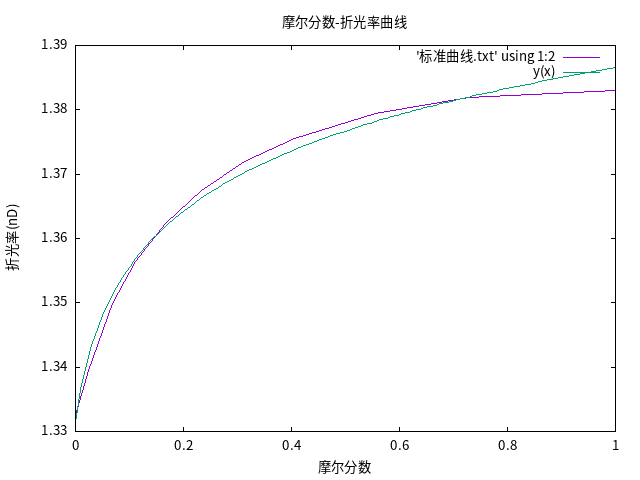
\includegraphics[width=.9\linewidth]{../data/标准曲线-对数曲线拟合.png}
\caption{\label{fig:orgdbf146d}对数曲线拟合结果}
\end{figure}
误差如下:
\begin{verbatim}
After 73 iterations the fit converged.
final sum of squares of residuals : 3.01193e-05
rel. change during last iteration : -1.25707e-06

degrees of freedom    (FIT_NDF)                        : 7
rms of residuals      (FIT_STDFIT) = sqrt(WSSR/ndf)    : 0.00207431
variance of residuals (reduced chisquare) = WSSR/ndf   : 4.30275e-06

Final set of parameters            Asymptotic Standard Error
=======================            ==========================
k               = 0.0146429        +/- 0.002306     (15.75%)
a               = 1.58346          +/- 1776         (1.121e+05%)
b               = 0.0374348        +/- 41.99        (1.122e+05%)
c               = 1.37943          +/- 16.41        (1190%)

correlation matrix of the fit parameters:
		k      a      b      c      
k               1.000 
a               0.855  1.000 
b               0.856  1.000  1.000 
c              -0.855 -1.000 -1.000  1.000 
\end{verbatim}
\[
     y=0.01464\ln(1.5835x+0.03743)+1.3794
     \]
目前来看对数曲线拟合的结果是最好的
\item 根号曲线拟合
\label{sec:orge2f1991}
拟合结果见 Fig 7.3
\begin{figure}[htbp]
\centering
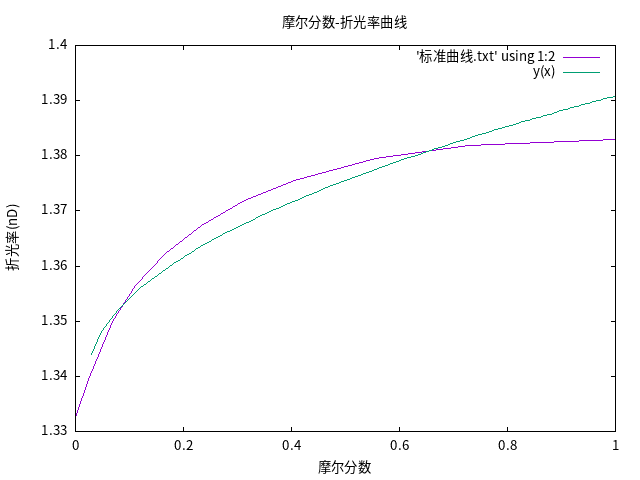
\includegraphics[width=.9\linewidth]{../data/标准曲线-根号曲线拟合.png}
\caption{\label{fig:orge54bb98}根号曲线拟合结果}
\end{figure}
误差计算如下:
\begin{verbatim}
After 163 iterations the fit converged.
final sum of squares of residuals : 0.000182336
rel. change during last iteration : -5.88249e-07

degrees of freedom    (FIT_NDF)                        : 7
rms of residuals      (FIT_STDFIT) = sqrt(WSSR/ndf)    : 0.00510372
variance of residuals (reduced chisquare) = WSSR/ndf   : 2.60479e-05

Final set of parameters            Asymptotic Standard Error
=======================            ==========================
k               = 0.0462516        +/- 0.005027     (10.87%)
a               = 1.23587          +/- 0.03517      (2.846%)
b               = -0.0302804       +/- 0.06359      (210%)
c               = 1.34005          +/- 0.004874     (0.3637%)

correlation matrix of the fit parameters:
#                k      a      b      c      
k               1.000 
a               0.448  1.000 
b               0.259  0.501  1.000 
c              -0.747 -0.691 -0.735  1.000 

\end{verbatim}
\[
     y=0.04625\sqrt{1.2359x-0.03028}+1.3401
     \]
拟合效果较差

\item 高(四)次曲线拟合
\label{sec:orgda54842}
拟合结果见 Fig 7.4
\begin{figure}[htbp]
\centering
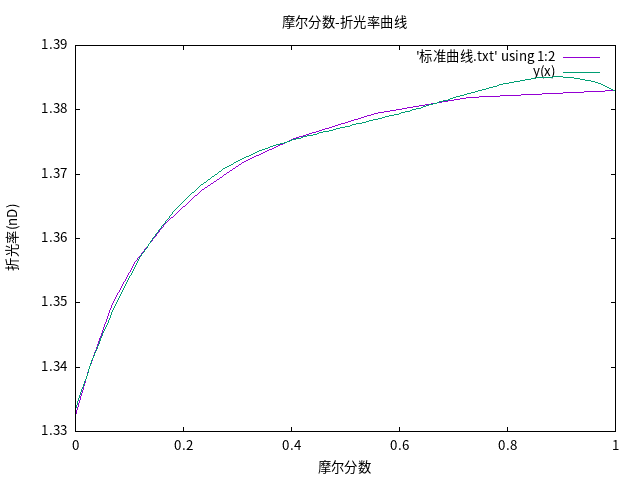
\includegraphics[width=.9\linewidth]{../data/标准曲线-四次曲线拟合.png}
\caption{\label{fig:org7f510b5}四次曲线拟合结果}
\end{figure}
误差计算如下:
\begin{verbatim}
After 6 iterations the fit converged.
final sum of squares of residuals : 5.55343e-06
rel. change during last iteration : -2.31074e-13

degrees of freedom    (FIT_NDF)                        : 6
rms of residuals      (FIT_STDFIT) = sqrt(WSSR/ndf)    : 0.000962066
variance of residuals (reduced chisquare) = WSSR/ndf   : 9.25572e-07

Final set of parameters            Asymptotic Standard Error
=======================            ==========================
a               = -0.312369        +/- 0.05993      (19.19%)
b               = 0.743501         +/- 0.1158       (15.57%)
c               = -0.645425        +/- 0.0697       (10.8%)
d               = 0.263831         +/- 0.01417      (5.373%)
e               = 1.33338          +/- 0.0007474    (0.05605%)

correlation matrix of the fit parameters:
#                a      b      c      d      e      
a               1.000 
b              -0.994  1.000 
c               0.962 -0.986  1.000 
d              -0.857  0.903 -0.959  1.000 
e               0.477 -0.527  0.610 -0.760  1.000 

\end{verbatim}
\[
     y=-0.3124x^{4}+0.7435x^{3}--0.6454x^{2}+ 0.2638x+1.3334
     \]
拟合效果和对数曲线相近,而这种方法引入的参数过多,并不能反应其内部规律
\end{enumerate}

\section{根据标准曲线和折光率推算摩尔分数}
\label{sec:org40314a3}
根据以上的拟合结果我们采用对数曲线进行计算
\[
    y=0.01464\ln(1.5835x+0.03743)+1.3794
    \]
它的反函数为:
\[
    x=(\exp((y-1.3794)/0.01464)-0.03743)/1.5835
    \]
其中x为醇的摩尔分数,y为折光率
\begin{enumerate}
\item 醇加水数据
\label{sec:orgb7b6432}
\begin{table}[htbp]
\caption{\label{tab:org962982a}醇加水数据计算}
\centering
\begin{tabular}{rrrrr}
气相(nD) & 液相(nD) & 气相摩尔分数 & 液相摩尔分数 & t\textsubscript{均}(\textsuperscript{o}C)\\
\hline
1.3831 & 1.3830 & 0.7895 & 0.7839 & 97.4327\\
1.3827 & 1.3831 & 0.7675 & 0.7895 & 95.6727\\
1.3811 & 1.3830 & 0.6856 & 0.7839 & 93.1170\\
1.3784 & 1.3825 & 0.5662 & 0.7568 & 90.6583\\
1.3779 & 1.3816 & 0.5464 & 0.7103 & 89.1757\\
1.3772 & 1.3803 & 0.5198 & 0.6479 & 88.3533\\
1.3766 & 1.3779 & 0.4979 & 0.5464 & 88.0267\\
1.3765 & 1.3766 & 0.4944 & 0.4979 & 88.0063\\
1.3764 & 1.3764 & 0.4909 & 0.4909 & 87.9963\\
1.3764 & 1.3763 & 0.4909 & 0.4874 & 87.9827\\
\end{tabular}
\end{table}

\item 水加醇数据
\label{sec:org4322930}
\begin{table}[htbp]
\caption{\label{tab:org3172747}水加醇数据计算}
\centering
\begin{tabular}{rrrrr}
气相(nD) & 液相(nD) & 气相摩尔分数 & 液相摩尔分数 & t\textsubscript{均}(\textsuperscript{o}C)\\
\hline
1.3325 & 1.3325 & 0.0020 & 0.0020 & 100.4657\\
1.3488 & 1.3326 & 0.0545 & 0.0022 & 100.4237\\
1.3575 & 1.3327 & 0.1179 & 0.0024 & 99.8970\\
1.3641 & 1.3344 & 0.1984 & 0.0056 & 99.0580\\
1.3696 & 1.3354 & 0.2997 & 0.0076 & 96.3293\\
1.3741 & 1.3381 & 0.4161 & 0.0140 & 91.2610\\
1.3758 & 1.3664 & 0.4702 & 0.2362 & 88.1557\\
1.3762 & 1.3741 & 0.4839 & 0.4161 & 88.0223\\
1.3764 & 1.3767 & 0.4909 & 0.5015 & 88.0443\\
1.3764 & 1.3760 & 0.4909 & 0.4770 & 88.0373\\
1.3764 & 1.3763 & 0.4909 & 0.4874 & 88.0377\\
\end{tabular}
\end{table}
\end{enumerate}

\section{摩尔分数沸点曲线}
\label{sec:orgcee0405}
如表格7.4所示,我们将表7.3和表7.2的摩尔分数和沸点部分进行了合并,
之后使用特鲁顿规则及克劳修斯-克拉贝龙公式,根据Tab 6.1 进行校正,
并利用它作图得到图7.5,考虑到其中可能存在的坏点,我对曲线利用bezier方法进行了平滑化,
得到了图7.6所示的结果,可以明显地看出其中的共沸点,数据处理效果良好
\begin{table}[htbp]
\caption{\label{tab:orgf03926d}摩尔分数-沸点曲线数据}
\centering
\begin{tabular}{rrrr}
气相摩尔分数 & 液相摩尔分数 & t\textsubscript{均}(\textsuperscript{o}C) & t\textsubscript{沸}(\textsuperscript{o}C)\\
\hline
0.0020 & 0.0020 & 100.4657 & 100.4664\\
0.0545 & 0.0022 & 100.4237 & 100.4244\\
0.1179 & 0.0024 & 99.8970 & 99.8977\\
0.1984 & 0.0056 & 99.0580 & 99.0587\\
0.2997 & 0.0076 & 96.3293 & 96.3300\\
0.4161 & 0.0140 & 91.2610 & 91.2617\\
0.4702 & 0.2362 & 88.1557 & 88.1564\\
0.4839 & 0.4161 & 88.0223 & 88.0230\\
0.4909 & 0.5015 & 88.0443 & 88.0450\\
0.4909 & 0.4770 & 88.0373 & 88.0380\\
0.4909 & 0.4874 & 88.0377 & 88.0384\\
0.4909 & 0.4909 & 87.9963 & 87.9970\\
0.4909 & 0.4874 & 87.9827 & 87.9834\\
0.4944 & 0.4979 & 88.0063 & 88.0070\\
0.4979 & 0.5464 & 88.0267 & 88.0274\\
0.5198 & 0.6479 & 88.3533 & 88.3540\\
0.5464 & 0.7103 & 89.1757 & 89.1764\\
0.5662 & 0.7568 & 90.6583 & 90.6590\\
0.6856 & 0.7839 & 93.1170 & 93.1177\\
0.7675 & 0.7895 & 95.6727 & 95.6734\\
0.7895 & 0.7839 & 97.4327 & 97.4334\\
\end{tabular}
\end{table}

\begin{figure}[htbp]
\centering
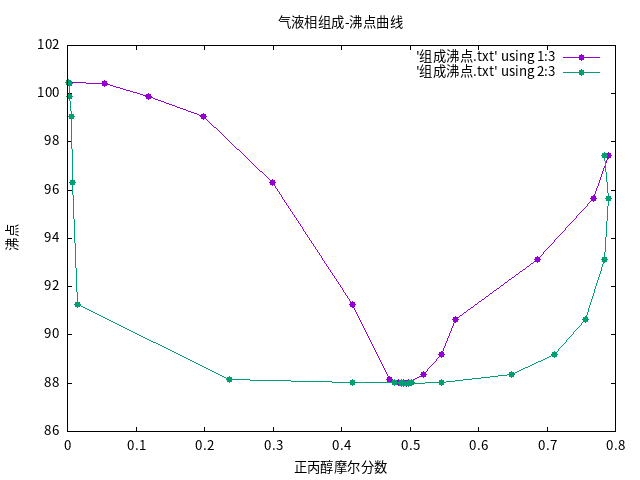
\includegraphics[width=.9\linewidth]{../data/气液相组成-沸点曲线.png}
\caption{\label{fig:orgefd6169}水-正丙醇体系气液相图}
\end{figure}

\begin{figure}[htbp]
\centering
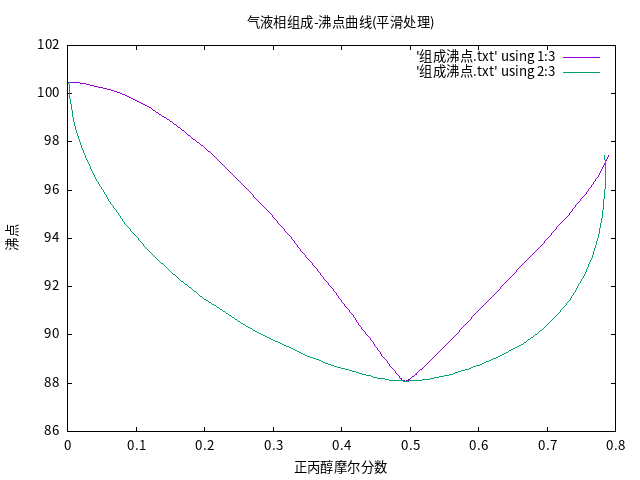
\includegraphics[width=.9\linewidth]{../data/气液相组成-沸点曲线(平滑处理).png}
\caption{\label{fig:org8cbb44f}水-正丙醇体系气液相图(平滑处理)}
\end{figure}




可以看出在正丙醇摩尔分数为0.4331时(考虑到本实验所用的标准曲线拟合有一定的偏差,
这里的值用的是标准曲线折光度相近的两点线性拟合的结果,见下),达到了最低沸点87.9827\textsuperscript{o}C,此时
正丙醇的质量百分数为
\[
    w%=\frac{0.4331*60.09}{(1-0.4331)*18.01+0.4331*60.09}=71.82%
    \]

\[
    (1.3763-1.3756)/(1.3795-1.3756)\times (0.5553-0.4064)+0.4064=0.4331
    \]
\end{document}
